\section{Ejemplo de proceso de selección}\label{Ap:Eje Seleccion}

Para este proceso de selección en particular, se hace referencia a las opciones mostradas en la tabla \ref{tab:Tar_Des}.

En la siguiente tabla se presenta una breve comparación entre las diversas opciones que se han considerado para el proyecto, resaltando las características más importantes para el funcionamiento del sistema. 

Para ser considera alguna de las opciones, era necesario que fuera un tarjeta de desarrollo que sea capaz de trabajar sin problemas las 72 horas que dura el proceso de compostaje. Además de contar con un gran numero de pines y de puertos de comunicación para realizar la conexión con los sensores, botones y elementos electrónicos necesarios.

\begin{table}[h!]
    \centering
    \caption{Tarjetas de desarrollo}
    \resizebox{16cm}{!}{
        \begin{tabular}{ |c|c|c|c|c| } 
            \hline
                Modelo & ESP32 & Raspberry Pi Pico & Arduino Nano & Arduino Mega \\ \hline
                Imagen & 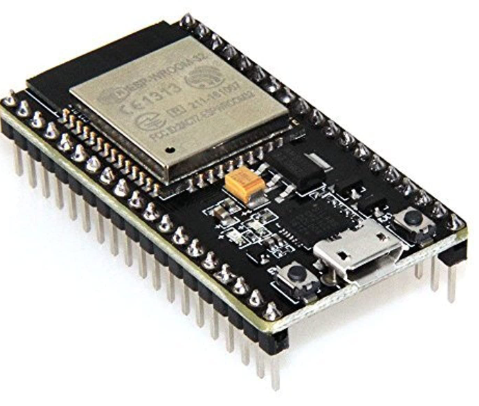
\includegraphics[scale=0.15]{images/Capitulo 4/3.1.1/S1/esp.png} & 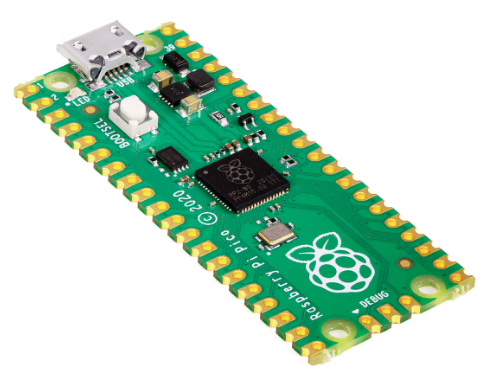
\includegraphics[scale=0.15]{images/Capitulo 4/3.1.1/S1/rasp.png} &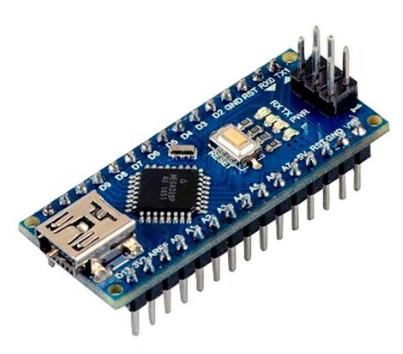
\includegraphics[scale=0.15]{images/Capitulo 4/3.1.1/S1/nano.png} & 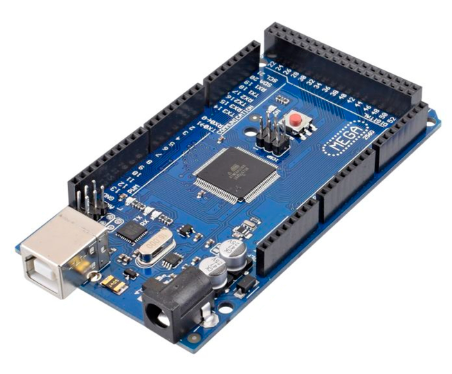
\includegraphics[scale=0.15]{images/Capitulo 4/3.1.1/S1/mega.png} \\ \hline
                Microcontrolador & Tensilica Xtensa 32-bit LX6 & RP2040 & ATMEGA328P & ATmega2560 \\
                Alimentación & 3.3 V & 3.3 V & 5 V & 5 V \\
                Corriente de operación & 20 a 240 mA & 1.3 a 93.5 mA & 20 a 40 mA & 20 a 50 mA \\
                Pines de comunicación & GPIO 24 & GPIO 26 & 14 Digitales 8 Analógicas & 54 Digitales y 16 Analógicas \\
                Dimensiones & 51 x 23 mm & 51 x 21 mm & 18 x 45 mm & 101.52 x 53.3 mm \\
                WIFI & Si & No & No & No \\
                Bluetooth & Si & No & No & No \\
                Frecuancia de trabajo & 240 Mhz & 133 MHz & 16 MHz & 16 MHz \\
                Precio & \$ 138.00 & \$ 114.00 & \$ 118.00 & \$ 272.00 \\
             \hline
        \end{tabular}
        }
    \label{tab:Tar_Des}%
\end{table}

Para la matriz de decisión, se tomaron en cuenta los siguientes requisitos:

\begin{itemize}
    \item Precio
    \item Accesibilidad
    \item Numero de pines
    \item Dimensiones
    \item Wifi
    \item Frecuencia de trabajo
\end{itemize}

La ponderación se realizo utilizando los siguientes valores para la evaluación de las diferentes opciones se encuentran en la tabla \ref{tab: Val des ap4}. Esta tiene fija un valor numérico que permite realizar un análisis cuantitativo para tomar alguna decisión de manera mas consciente

\begin{table}
    \centering
\caption{Ponderaciones para la matriz de decisión}
\label{tab: Val des ap4}
    \begin{tabular}{|c |c |} \hline 
         \multicolumn{2}{|c|}{Valores de ponderación}\\ \hline
         Excelente& 5\\ \hline
         Bueno& 4\\ \hline
         Regular& 3\\ \hline
 Malo&2\\ \hline
    \end{tabular}  
\end{table}

Se realizo la tabla de decisión para analizar las opciones mostradas en la tabla \ref{tab:Tar_Des} entonces se obtuvieron los valores que se muestran en la tabla\ref{tab:toma des tar des}


\begin{table}
    \centering
\caption{Ejemplo de toma de decisión de la tarjeta de desarrollo}
\label{tab:toma des tar des}
\resizebox{!}{17 cm}{
\begin{turn}{90}
    \begin{tabular}{|c|c|c|c|c|c|l|l|} \hline  
         Tarjeta de desarrollo&  \multicolumn{7}{|c|}{Caracteristica}\\ \hline  
         &  Precio&  Accesibilidad&  Numero de pines&  Dimensiones& Wifi & Frecuencia de trabajo&Total\\ \hline  
         \rowcolor[rgb]{ 1,  1,  0} 
 ESP32&  4&  5&  5&  4&  5& 5&28\\ \hline  
         Raspberry Pi Pico&  5&  3&  5&  4&  2& 4&23\\ \hline  
         Arduino Nano&  5&  5&  3&  5&  2& 2&22\\ \hline  
 Arduino Mega& 3& 5& 5& 3& 2& 2&20\\ \hline 
    \end{tabular}
    
    \end{turn}
    }
\end{table}

Con este proceso de toma de decisiones, se llego a la conclusión de que la tarjeta ESP32 es la que mejor se adapta a las necesidades del proyecto, es la opción que esta resaltada de la tabla \ref{tab:toma des tar des}
